%!TEX program = xelatex
% 完整编译: xelatex -> biber/bibtex -> xelatex -> xelatex
\documentclass[lang=cn,a4paper,newtx,bibend=bibtex]{elegantpaper}
\usepackage{tikz}
\usepackage{pgfplots}
\usepackage{float}

\title{Programming Report of Chapter 2}
\author{张志心 \ 混合2106}

\date{\zhdate{2023/10/08}}

% \qedhere to make the square straight after

\usepackage{array}
\usepackage{tcolorbox}

\newtcolorbox{prob}[1][]{
  colframe=gray,
  colback=white,
  boxrule=1.5pt, % 控制外边框线的宽度
  sharp corners, % 使用直角边框
  fonttitle=\bfseries,
  title=#1
}

\newcommand{\ccr}[1]{\makecell{{\color{#1}\rule{1cm}{1cm}}}}

\addbibresource[location=local]{reference.bib}

\begin{document}

\maketitle

\section{设计思路}

\subsection{多项式函数类}

要使用多项式函数类,请调用相关库 \lstinline[language=C++]{#include "function.hpp"}。

多项式函数类 \lstinline[language=C++]{Poly_n<Type>} 继承于
函数类 \lstinline[language=C++]{Function<Type, Type>}。默认情况为 $\text{double}\to\text{double}$ 的多项式函数。多项式函数类包含
的成员变量有两个,\lstinline[language=C++]{int16_t n;} 和 \lstinline[language=C++]{vector<Type> coef;}
 分别表示多项式的次数加一的值(为了方便遍历多项式的系数)和系数。


\begin{lstlisting}[language=C++]
  template<class Type=double>class Poly_n: public Function<Type, Type>
\end{lstlisting}

除了默认构造以及拷贝构造方法之外,还定义两种多项式函数的构造方法,具体如下,
分别用于临时指定次数的多项式以及特定多项式的构造。

\begin{lstlisting}[language=C++]
  explicit Poly_n(int16_t n) : n(n), coef(n) {}
  explicit Poly_n(const vector<Type>& a) : n(a.size()), coef(a) {}
\end{lstlisting}

多项式函数类包含的特有方法有:多项式加、减、数乘运算,多项式乘法(采用朴素 $O(n^2)$ 复杂度做法)、
获取导函数等。此外,为了方便使用多项式函数的表达式进行计算机绘图,
还定义了如下三个函数,用于将多项式的表达式以字符串格式保存为可被tikz、latex、python识别的格式。

\begin{lstlisting}[language=C++]
  const std::string to_tikz() const;
  const std::string to_latex() const;
  const std::string to_python() const;
\end{lstlisting}


\subsection{多项式插值}

要使用插值的相关类或函数,请调用库 \lstinline[language=C++]{#include "Interpolation.hpp"},
多项式插值类以及相关接口函数均已封装在命名空间 \lstinline{namespace polynomial_interpolation} 中。

多项式插值类 \lstinline[language=C++]{Polynomial_Interpolation<Type>} 
为基本模版类,主要成员包括输入的点与点值序列(
\lstinline[language=C++]{vector<Type> x, y;}),差商表(
\lstinline[language=C++]{vector<Type> d_table;})
以及插值多项式的次数(\lstinline[language=C++]{int16_t n;})。请使用点与点值序列(用 \lstinline[language=C++]{std::vector<Type>} 存储)
来构造多项式插值类,构造方法如下:

\begin{lstlisting}[language=C++]
  Polynomial_Interpolation (const vector<Type> &x, const vector<Type> &y) 
                            : x(x), y(y), n(x.size()-1) {}
\end{lstlisting}

使用 \lstinline[language=C++]{Poly_n<Type> Polynomial_Interpolation::solve()} 来求解多项式插值函数。
求解过程为,先计算差商表,然后根据下式计算插值函数。

\[
  p_n(x) = \sum_{k=0}^n [x_0, \cdots, x_k]f \pi_k(x), ~~~~~~~~~~~~~~~~~~~~~~~~\pi_1(x) = 1, \pi_k(x) = \prod_{j=0}^{k-1} (x-x_j), k>1
\]

注意,由于插商表实际有用的位置只有对角线元素,且实际计算的时候可以通过数组滚动达到空间
复杂度为 $O(n)$,因此项目中的差商表为一维线性表(\lstinline[language=C++]{std::vector<Type>} 类型)。

计算差商表的方法由于插值类型的不同,有不同的定义,
因此基类中 \lstinline[language=C++]{void Polynomial_Interpolation::make_d_table()} 
仅仅为一个纯虚函数,而在其子类中再进行明确定义。

\subsubsection{Newton 插值}

Newton 插值法为多项式插值类的子类,
\begin{lstlisting}[language=C++]
  template<class Type=NUM>
  class Newton_Interpolation : public Polynomial_Interpolation<Type>;
\end{lstlisting}

调用示例子如下:
\begin{lstlisting}[language=C++]
  Newton_Interpolation sol(x, y);
  Poly_n<NUM> res = sol.solve();
\end{lstlisting}

在计算差商表的时候,按照列的顺序进行计算,
并且使用了滚动数组的方式,使得空间复杂度为 $O(n)$。
差商表的递推公式为

\[
  [x_i, \cdots, x_j] f = \dfrac{[x_i, \cdots, x_{j-1}]f
  - [x_{i+1}, \cdots, x_j]f}{x_i - x_j}.
\]

\begin{lstlisting}[language=C++]
  void make_d_table() {
      d_table = y; // the first column is equal to the value array : y
      for(int i = 1; i <= n; ++i) {
          for(int j = n; j>=i ; --j) {
              if(x[j-i]==x[j]) d_table[j] = d_table[j]/i;
              else d_table[j]=(d_table[j]-d_table[j-1])/(x[j]-x[j-i]);
          }
      }
  }
\end{lstlisting}

为牛顿插值添加了两类接口函数,用于求解均匀插值问题和切比雪夫插值问题。

\begin{lstlisting}[language=C++]
  template<class T=NUM>
  const Poly_n<T> Grid_Interpolation(const T& l, const T& r, 
                          const int16_t& n, const Function<T>& f) {
      vector<T> x(n+1), y(n+1);
      for(int i = 0; i <= n; ++i) x[i]=l+i*(r-l)/n, y[i]=f(x[i]);
      Newton_Interpolation<T> solver(x, y);
      return solver.solve();
  }
  template<class T=NUM>
  const Poly_n<T> Chebyshev_Interpolation (const T& l, const T& r, 
                          const int16_t& n, const Function<T>& f) {
      static const T Pi = acos(-1.); // 3.14159265358979323846 maybe more precise
      vector <T> x(n+1), y(n+1);
      for (int i = 0; i <= n; ++ i) x[i] = (l+r)/2+(r-l)/2*cos(Pi*(2*i+1)/(2*n+2)), y[i] = f(x[i]);
      Newton_Interpolation<T> solver(x, y);
      return solver.solve();
  }
\end{lstlisting}

\subsubsection{Hermite 插值}

Hermite 插值法为多项式插值类的子类,
\begin{lstlisting}[language=C++]
  template<class Type=NUM>
  class Hermite_Interpolation : public Polynomial_Interpolation<Type>;
\end{lstlisting}

Hermite 插值与 Newton 插值的构造方法相同,为了保证一致性,输入的点与点值序列 $x, y$ 应当长度相同,
对于 $f^(k)(x_i) = y_i^{(k)}, k=0, \cdots, K$ 的限制应当以 $\{(x_i, y_i^{(k)})\}_{k=0}^K$ 的形式对应且连续的放入 $x, y$ 中。

调用示例子如下:
\begin{lstlisting}[language=C++]
  Hermite_Interpolation sol(x, y);
  Poly_n<NUM> res = sol.solve();
\end{lstlisting}

差商表的计算,要判断当前要求的 $[x_i, \cdots, x_j]f$ 中 $x_i, \cdots, x_j$ 是否都相同。
如果是,则值为 $\dfrac{f^{(j-i)}(x_i)}{(j-i)!}$,否则等同于 Newton 插值法的计算公式。

\begin{lstlisting}[language=C++]
  void make_d_table() {
      vector<int16_t> start(n+1);
      d_table.resize(n+1);
      d_table[0] = y[0]; start[0] = 0;
      for(int i = 1; i <= n; ++i) {
          if(x[i] == x[i-1]) d_table[i] = d_table[i-1], start[i]=start[i-1];
          else d_table[i] = y[i], start[i] = i;
      }
      Type fac = 1.;
      for(int i = 1; i <= n; ++i, fac *= i) {
          for(int j = n; j>=i ; --j) {
              if(x[j-i]==x[j]) d_table[j] = y[start[j]+i]/fac;
              else d_table[j]=(d_table[j]-d_table[j-1])/(x[j]-x[j-i]);
          }
      }
  }
\end{lstlisting}


\section{求解结果}

以下程序使用 \lstinline[language=C++]{std::ostream << (const Poly_n<double> &p) const;}
输出多项式,其格式为:

\[
  \{\text{n = } N, \text{coef = } \{e_0, e_1, \cdots, e_{N-1}\}\},
\]
其中 $e_{i}$ 表示多项式 $x^i$ 的系数。具体输出结果参考 \lstinline{/tmp/result.txt},以下仅展示处理后的输出结果。

\subsection{问题B}

函数 $f(x) = \dfrac{1}{1+x^2}$,在 $[-5, 5]$ 区间上的均匀插值。
其中 $x_i = -5 + 10\dfrac{i}{n}, n = 2, 4, 6, 8$。

对于该问题,使用 Newton 插值方法求解得到的函数如下:

\begin{equation*}
  \begin{aligned}
    p_2(x) &= -0.0384615x^{2}+1 \\
    p_4(x) &= 0.00530504x^{4}-0.171088x^{2}+1 \\
    p_6(x) &= -0.000840633x^{6}+8.67362\mathrm{e}{-}19x^{5}+0.0335319x^{4}+2.08167\mathrm{e}{-}17x^{3}-0.351364x^{2}+2.77556\mathrm{e}{-}17x+1 \\
    p_8(x) &= 0.000137445x^{8}-0.00658016x^{6}+0.0981875x^{4}-6.93889\mathrm{e}{-}17x^{3}-0.528121x^{2}+2.77556\mathrm{e}{-}17x+1 \\
     \end{aligned}
\end{equation*}

将 $f(x)$ 以及 Newton 插值的拟合结果 $p_2(x)$, $p_4(x)$, $p_6(x)$, $p_8(x)$ 绘制图像如下:

\begin{figure}[htbp]
  \centering
  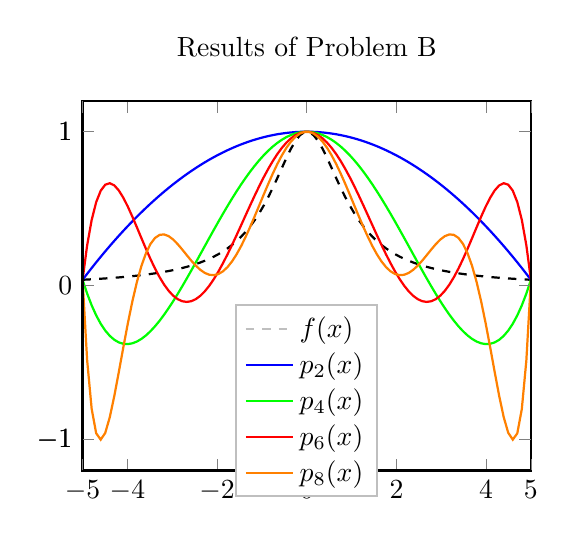
\begin{tikzpicture}
    \begin{axis}[
      xmin=-5, xmax=5,
      ymin=-1.2, ymax=1.2,
      width=0.6\textwidth,
      thick,
      samples=100,
      no markers,
      title={Results of Problem B},
      title style={yshift=1.5ex},
      legend style={at={(0.5,0.45)},anchor=north, draw=gray!50},
      legend cell align={left},
      axis on top,
      extra x ticks={-5, 5},
      extra y ticks={-1, 1},
    ]
      \addplot[domain=-5:5, dashed, thick] {1/(1+x^2)}; % f(x)
      \addplot[domain=-5:5, blue] {-0.0384615*x^2+1}; % p2(x)
      \addplot[domain=-5:5, green] {0.00530504*x^4-0.171088*x^2+1}; % p4(x)
      \addplot[domain=-5:5, red] {-0.000840633*x^6+8.67362e-19*x^5+0.0335319*x^4+2.08167e-17*x^3-0.351364*x^2+2.77556e-17*x+1}; % p6(x)
      \addplot[domain=-5:5, orange] {0.000137445*x^8-0.00658016*x^6+0.0981875*x^4-6.93889e-17*x^3-0.528121*x^2+2.77556e-17*x+1}; % p8(x)
  
      \legend{$f(x)$, $p_2(x)$, $p_4(x)$, $p_6(x)$, $p_8(x)$}
    \end{axis}
  \end{tikzpicture}
  \end{figure}

观察图像可以发现,随着 $n$ 的增大,插值多项式结果在 $[-2, 2]$ 
区间上的拟合效果越来越好,然而在 $\vert x\vert \ge 2$ 位置的振荡明显严重,
产生 Runge 现象。


\subsection{问题C}

函数 $f(x) = \dfrac{1}{1+25x^2}$,在 $[-1, 1]$ 区间上的切比雪夫插值。
其中 $x_i = -1 + 2\dfrac{i}{n}, n = 5, 10, 15, 20$。

对于该问题,使用 Newton 插值方法求解得到的函数见 \lstinline{/tmp/result.txt}。

将 $f(x)$ 以及 Newton 插值的拟合结果 $p_5(x)$, $p_{10}(x)$, $p_{15}(x)$, $p_{20}(x)$ 绘制图像如下:

\begin{figure}[H]
  \centering
  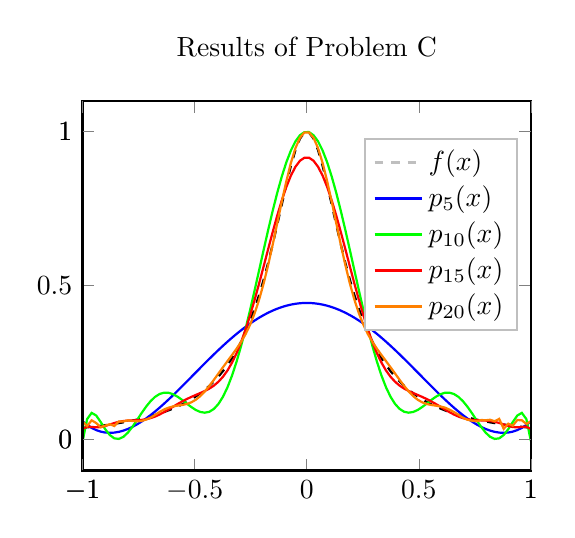
\begin{tikzpicture}
    \begin{axis}[
      xmin=-1, xmax=1,
      ymin=-0.1, ymax=1.1,
      width=0.6\textwidth,
      thick,
      samples=100,
      no markers,
      title={Results of Problem C},
      title style={yshift=1.5ex},
      legend style={at={(0.8,0.9)},anchor=north, draw=gray!50},
      legend cell align={left},
      axis on top,
      extra x ticks={-1, 1},
      extra y ticks={0, 1},
    ]
      \addplot[domain=-1:1, dashed, thick] {1/(1+25*x^2)}; % f(x)
      \addplot[domain=-1:1, blue] {-5.17224e-16*x^5+0.711567*x^4+2.9326e-16*x^3-1.09581*x^2+1.63088e-16*x+0.444089}; % p5(x)
      \addplot[domain=-1:1, green] {-46.6329*x^10+3.55271e-14*x^9+130.106*x^8-4.26326e-14*x^7-133.445*x^6+1.56319e-13*x^5+61.443*x^4-2.13163e-14*x^3-12.4765*x^2+1.77636e-15*x+1}; % p10(x)
      \addplot[domain=-1:1, red] {5.85464e-13*x^15-108.93*x^14-2.33045e-12*x^13+440.077*x^12+2.57202e-12*x^11-725.649*x^10-5.15846e-12*x^9+628.141*x^8+7.81847e-13*x^7-305.961*x^6-3.69476e-13*x^5+83.7238*x^4+4.86983e-14*x^3-12.2846*x^2-1.77185e-15*x+0.916893}; % p15(x)
      \addplot[domain=-1:1, orange] {6466.55*x^20-4.54747e-12*x^19-34208.1*x^18+7.27596e-11*x^17+77754.5*x^16+1.30967e-10*x^15-99300.1*x^14+8.00355e-11*x^13+78236.3*x^12-1.20053e-10*x^11-39333.3*x^10-4.00178e-11*x^9+12635.6*x^8+2.50111e-12*x^7-2537.27*x^6-1.08002e-12*x^5+306.629*x^4-2.66454e-14*x^3-21.7623*x^2+2.498e-15*x+1}; % p20(x)
  
      \legend{$f(x)$, $p_{5}(x)$, $p_{10}(x)$, $p_{15}(x)$, $p_{20}(x)$}
    \end{axis}
  \end{tikzpicture}
  \end{figure}

观察图像可以发现,随着 $n$ 的增大,插值多项式的拟合效果越来越好,
并且振荡幅度越来越微弱,Runge 现象被削弱。


\subsection{问题D}

根据题意可知,待插值函数满足:

\begin{center}
  \begin{tabular}{|c|c|c|c|c|c|}
    \hline
    $x$ & 0 & 3 & 5 & 8 & 13 \\
    \hline
    $f(x)$ & 0 & 225 & 383 & 623 & 993 \\
    \hline
    $f'(x)$ & 75 & 77 & 80 & 74 & 72 \\
    \hline
  \end{tabular}
  \end{center}

将 $x=0,3,5,8,13$ 处的函数值和导数值代入 Hermite 插值,得到结果为:
\[
  p(x)=-2.02236\mathrm{e}{-}05x^{9}+0.00104059x^{8}-0.0218757x^{7}+0.243041x^{6}-1.5383x^{5}+5.50812x^{4}-10.0953x^{3}+7.16191x^{2}+75x
\]
\[
  p'(x)=-0.000182013x^{8}+0.00832472x^{7}-0.15313x^{6}+1.45825x^{5}-7.69148x^{4}+22.0325x^{3}-30.2859x^{2}+14.3238x+75
\]

\begin{enumerate}
  \item 根据插值结果,$p(10)=742.503, p'(10)=48.3817$,分别为时间为 $10$ 时位移与速度的估计值。
  \item $p'(x)$ 的图像如下:
  \begin{figure}[htbp]
    \centering
    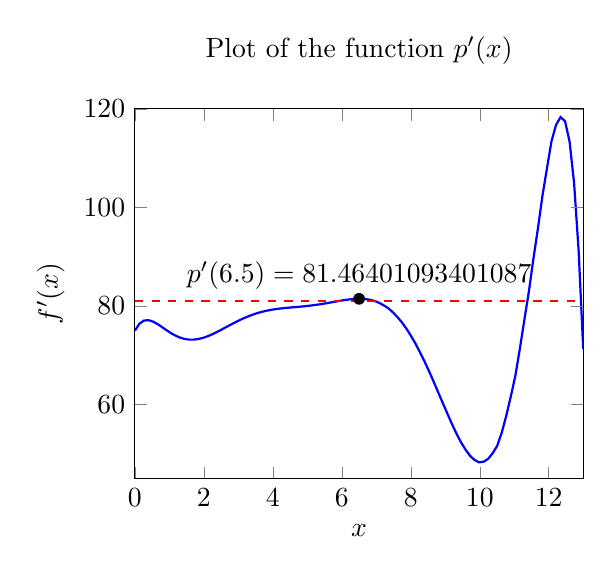
\begin{tikzpicture}
      \begin{axis}[
        xlabel={$x$},
        ylabel={$f'(x)$},
        ymin=45, ymax=120,
        xmin=0, xmax=13,
        samples=100,
        title={Plot of the function $p'(x)$},
        title style={yshift=1.5ex},
        legend cell align={left},
        axis on top,
        extra x ticks={50, 120},
        extra y ticks={0, 13},
        width=0.6\textwidth,
      ]
        \addplot[domain=0:13, blue, thick] {-0.000182013*x^8 + 0.00832472*x^7 - 0.15313*x^6 + 1.45825*x^5 - 7.69148*x^4 + 22.0325*x^3 - 30.2859*x^2 + 14.3238*x + 75};
        \draw[dashed, red] (axis cs:0,81) -- (axis cs:13,81) node[right] {$y=81$};
      
        \node[circle,fill,inner sep=1.5pt] at (axis cs:6.5, {(-0.000182013*(6.5)^8 + 0.00832472*(6.5)^7 - 0.15313*(6.5)^6 + 1.45825*(6.5)^5 - 7.69148*(6.5)^4 + 22.0325*(6.5)^3 - 30.2859*(6.5)^2 + 14.3238*6.5 + 75)}) {};
        \node[above] at (axis cs:6.5, {(-0.000182013*(6.5)^8 + 0.00832472*(6.5)^7 - 0.15313*(6.5)^6 + 1.45825*(6.5)^5 - 7.69148*(6.5)^4 + 22.0325*(6.5)^3 - 30.2859*(6.5)^2 + 14.3238*6.5 + 75)}) {$p'(6.5)=81.46401093401087$};
    
      \end{axis}
    \end{tikzpicture}
  \end{figure}
\end{enumerate}

根据图像,$p'(x)$ 在 $x=6.5$ 附近超过了限速 $81 \text{ ft}$,
而在 $x=12$ 附近速度突增再突减,峰值远远超过了 $81 \text{ ft}$。
这显然不太可能与实际情况相符,可能是由于高次多项式的振荡。

这说明插值方法在个别点处的拟合结果的相对误差可能会很大。
要进一步提高拟合精度,可能需要更多的点或者采用分段插值。

\subsection{问题E}
  
根据已知信息,

\begin{center}
  \begin{tabular}{|c|c|c|c|c|c|c|c|}
    \hline
    $x$ & 0 & 6 & 10 & 13 & 17 & 20 & 28 \\
    \hline
    $f_1(x)$ & 6.67 & 17.3 & 42.7 & 37.3 & 30.1 & 29.3 & 28.7 \\
    \hline
    $f_2(x)$ & 6.67 & 16.1 & 18.9 & 15.0 & 10.6 & 9.44 & 8.89\\
    \hline
  \end{tabular}
  \end{center}

使用 Newton 插值,得到结果为:

\begin{equation*}
\begin{aligned}
p_1(x) &= 4.1477\mathrm{e}{-}05x^{6}-0.00371557x^{5}+0.128281x^{4}-2.11512x^{3}+16.2855x^{2}-43.0127x+6.67 \\
p_2(x) &= 8.6768\mathrm{e}{-}06x^{6}-0.000777473x^{5}+0.0265858x^{4}-0.424283x^{3}+2.98227x^{2}-5.85018x+6.67
\end{aligned}
\end{equation*}

\begin{enumerate}
  \item 插值结果 $p_1(x), p_2(x)$ 的图像如下:
  
  \begin{figure}[H]
    \centering
    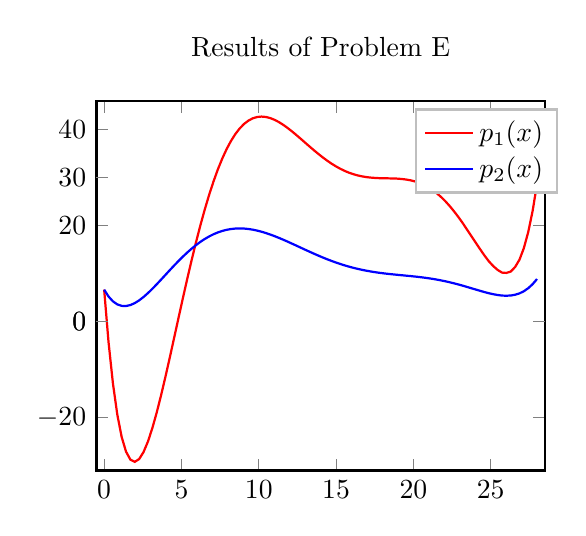
\begin{tikzpicture}
      \begin{axis}[
        xmin=-0.5, xmax=28.5,
        ymin=-31, ymax=46,
        width=0.6\textwidth,
        thick,
        samples=100,
        no markers,
        title={Results of Problem E},
        title style={yshift=1.5ex},
        legend style={at={(0.87,0.98)},anchor=north, draw=gray!50},
        legend cell align={left},
        axis on top,
        extra x ticks={-30, 40},
        extra y ticks={0, 30},
      ]
        \addplot[domain=0:28, red] {4.1477e-05*x^6-0.00371557*x^5+0.128281*x^4-2.11512*x^3+16.2855*x^2-43.0127*x+6.67};
        \addplot[domain=0:28, blue] {8.6768e-06*x^6-0.000777473*x^5+0.0265858*x^4-0.424283*x^3+2.98227*x^2-5.85018*x+6.67};
        \legend{$p_1(x)$, $p_2(x)$};
      \end{axis}
    \end{tikzpicture}
    \end{figure}

    $f_1(x)$ 的插值结果 $p_1(x)$ 在 $x=2$ 附近存在较大振荡,
    导致函数值出现在负数区域,与实际情况不符合。
    可能原因是 $f_1(x)$ 的已知点值的变换幅度过大,
    要更准确的拟合函数,可能需要更高次的函数(因此需要更多的点)。
    $f_2(x)$ 的插值结果与实际走势基本吻合。
  
  \item 根据插值结果估计 15 天后的两类幼虫质量为 
  $p_1(43) = 14640.3, p_2(43) = 2981.48$,
  这个值远高于实际可能的情况。
  可以发现两个函数在 $x\ge 25$ 之后都有快速增长的趋势,
  这是因为提供的用于插值的点都在 $[0, 28]$ 范围内,
  对插值范围之外的点的估计不可靠。
  由于两个函数都是一个最高次项系数大于0的六次多项式,
  因此当 $x$ 远离插值范围后,都会快速增长。
  
\end{enumerate}
  
\nocite{*}
\printbibliography[heading=bibintoc, title=\ebibname]

% \appendix
% % \appendixpage
% \addappheadtotoc

\end{document}
